\documentclass[border=3pt]{standalone}
% Shared TikZ styles for the Ch. 3–8 diagrams (standalone PDFs); extends the Ch. 1 palette (s1_vs_llm_common.tex).
\usepackage[T1]{fontenc}
\usepackage{lmodern}
\usepackage[english]{babel}
\usepackage{amsmath,amssymb}
\usepackage{tikz}
\usetikzlibrary{shapes.geometric,shapes.misc,positioning,fit,arrows.meta,calc,backgrounds,decorations.pathreplacing,patterns}
\definecolor{ioFill}{HTML}{F1F0EC}\definecolor{ioLine}{HTML}{52514E}
\definecolor{modFill}{HTML}{E8F1FB}\definecolor{modLine}{HTML}{2A78D6}
\definecolor{decFill}{HTML}{ECE9F7}\definecolor{decLine}{HTML}{4A3AA7}
\definecolor{postFill}{HTML}{FFF6E0}\definecolor{postLine}{HTML}{EDA100}
\definecolor{okFill}{HTML}{EAF7F1}\definecolor{okLine}{HTML}{1BAF7A}
\definecolor{badFill}{HTML}{FDECEC}\definecolor{badLine}{HTML}{E34948}
\definecolor{nmFill}{HTML}{EFEAF8}\definecolor{nmLine}{HTML}{4A3AA7}
\definecolor{loopRed}{HTML}{E34948}\definecolor{clusterLine}{HTML}{9A9890}\definecolor{ink2}{HTML}{52514E}
\definecolor{orangeA}{HTML}{EB6834}
\tikzset{
  every node/.style={font=\small, align=center},
  io/.style={trapezium, trapezium left angle=72, trapezium right angle=108, trapezium stretches body,
             draw=ioLine, fill=ioFill, thick, inner sep=3pt, minimum height=2.4em},
  model/.style={rectangle, draw=modLine, fill=modFill, very thick, inner sep=4pt, minimum height=2.4em, text width=#1},
  model/.default=3.6cm,
  post/.style={rectangle, draw=postLine, fill=postFill, very thick, inner sep=4pt, minimum height=2.2em, text width=#1},
  post/.default=3.6cm,
  data/.style={cylinder, shape border rotate=90, aspect=0.18, draw=okLine, fill=okFill, very thick, inner sep=3pt, minimum height=2.6em, text width=#1},
  data/.default=2.4cm,
  decision/.style={diamond, aspect=2.1, draw=decLine, fill=decFill, very thick, inner sep=1pt},
  outcome/.style={rounded rectangle, draw=#1, thick, inner sep=4pt, minimum height=2em},
  arrow/.style={-{Latex[length=2mm]}, thick, ioLine},
  dashedarrow/.style={-{Latex[length=2mm]}, thick, ioLine, dashed},
  loop/.style={-{Latex[length=2.4mm]}, line width=1.4pt, loopRed},
  cluster/.style={draw=clusterLine, dashed, rounded corners=3pt, inner sep=7pt},
  clusterlabel/.style={font=\small\bfseries, text=ioLine},
  note/.style={font=\footnotesize, text=ink2},
  tok/.style={rectangle, draw=ioLine, fill=ioFill, thin, inner sep=2pt, minimum height=1.6em, font=\footnotesize},
  vmark/.style={rectangle, draw=orangeA, fill=postFill, thick, inner sep=2pt, minimum height=1.6em, font=\footnotesize\ttfamily},
}

\begin{document}
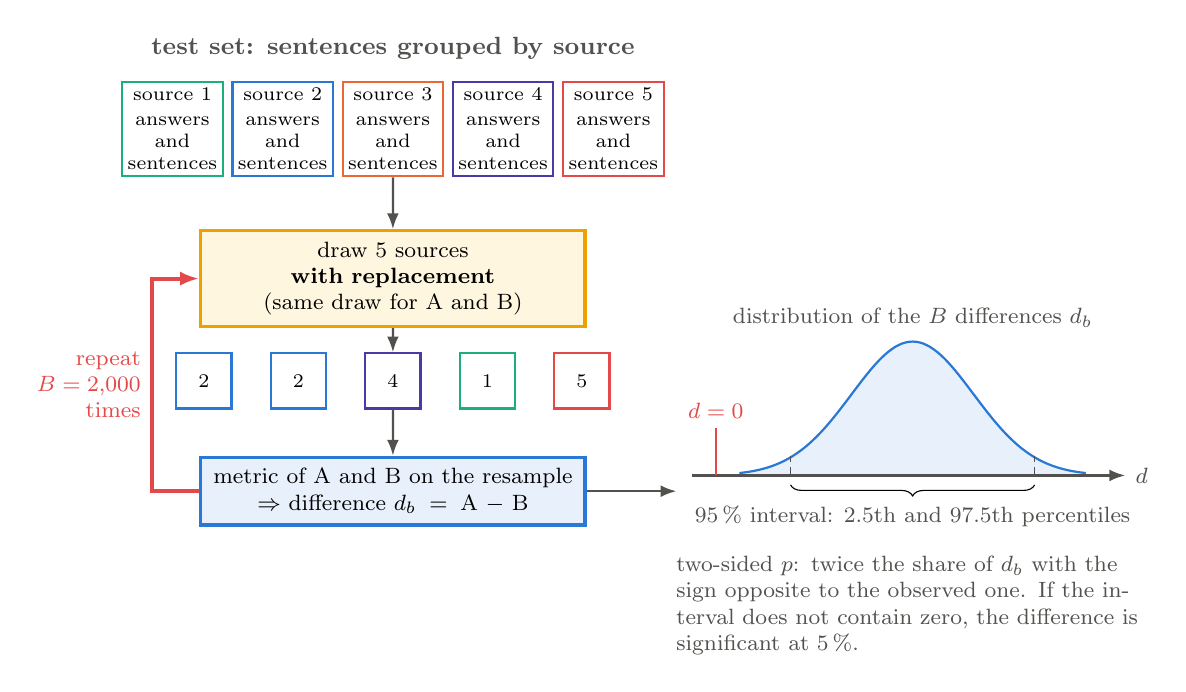
\begin{tikzpicture}
  \foreach \i/\c in {1/okLine,2/modLine,3/orangeA,4/decLine,5/badLine}
    \node[rectangle, draw=\c, thick, fill=white, minimum width=1.2cm, minimum height=1.2cm, inner sep=2pt, font=\scriptsize] (g\i) at ({(\i-1)*1.4},0) {source \i\\[1pt]answers\\and\\sentences};
  \node[clusterlabel, above=1.5mm of g3] {test set: sentences grouped by source};
  \node[post=4.6cm, font=\footnotesize] (rs) at (2.8,-1.9) {draw 5 sources \textbf{with replacement}\\(same draw for A and B)};
  \draw[arrow] (g3.south) -- (rs);
  \foreach \i/\c/\x in {2/modLine/0,2/modLine/1,4/decLine/2,1/okLine/3,5/badLine/4}
    \node[rectangle, draw=\c, thick, fill=white, minimum width=0.7cm, minimum height=0.7cm, font=\scriptsize] (r\x) at ({0.4+\x*1.2},-3.2) {\i};
  \draw[arrow] (rs) -- (r2);
  \node[model=4.6cm, font=\footnotesize] (dm) at (2.8,-4.6) {metric of A and B on the resample\\$\Rightarrow$ difference $d_b = \mathrm{A} - \mathrm{B}$};
  \draw[arrow] (r2) -- (dm);
  \draw[loop] (dm.west) -- ++(-6mm,0) |- node[pos=0.25, left, note, text=loopRed, align=right] {repeat\\$B = 2{,}000$\\times} (rs.west);
  \begin{scope}[shift={(9.4,-4.4)}]
    \fill[modFill] plot[domain=-2.2:2.2, samples=50, smooth] (\x, {1.7*exp(-\x*\x/1.2)}) -- (2.2,0) -- (-2.2,0) -- cycle;
    \draw[thick, modLine] plot[domain=-2.2:2.2, samples=50, smooth] (\x, {1.7*exp(-\x*\x/1.2)});
    \draw[thick, ioLine, -{Latex[length=2mm]}] (-2.8,0) -- (2.7,0) node[right, note] {$d$};
    \draw[densely dashed, ink2] (-1.55,0) -- (-1.55,0.25) (1.55,0) -- (1.55,0.25);
    \draw[decorate, decoration={brace, amplitude=4pt, mirror}] (-1.55,-0.12) -- node[below=4pt, note] {95\,\% interval: 2.5th and 97.5th percentiles} (1.55,-0.12);
    \draw[thick, badLine] (-2.5,0) -- (-2.5,0.6);
    \node[note, text=badLine, above=0mm] at (-2.5,0.6) {$d = 0$};
    \node[note] at (0,2.0) {distribution of the $B$ differences $d_b$};
    \node[note, text width=6.0cm, align=left, anchor=north] at (0,-0.9) {two-sided $p$: twice the share of $d_b$ with the sign opposite to the observed one. If the interval does not contain zero, the difference is significant at 5\,\%.};
  \end{scope}
  \draw[arrow] (dm.east) -- (6.4,-4.6);
\end{tikzpicture}
\end{document}
